\documentclass{article}
\usepackage{amsmath}
\usepackage{amssymb}
\usepackage{graphicx}
\usepackage{hyperref}
\usepackage[version=4]{mhchem}


\begin{document}
\section*{Problem}
As shown in the figure, \(A B / / C D . A D \perp A B . A D\) and \(B C\) meet at \(E\) such that \(E B=2 A C\). Show that \(\angle A C D=3 \angle B C D\).\\
\centering
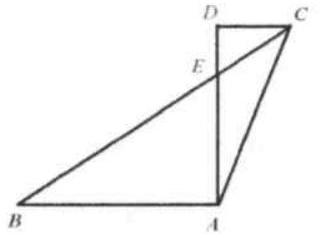
\includegraphics[width=\textwidth]{images/016(2).jpg}

\section*{Solution}
(C).\\
Draw \(D G \perp B C\) where \(G\) is on \(B C\). Let \(A C=x\) and \(G C=y\). We know that \(B C D\) is isosceles so \(B C=2 y\).\\
\centering
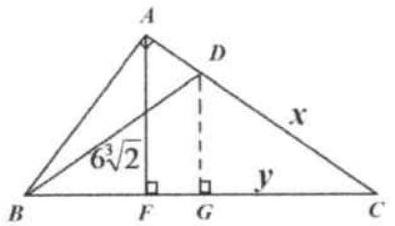
\includegraphics[width=\textwidth]{images/094(1).jpg}


Since \(\triangle D C G, \triangle A C F\), and \(\triangle B C A\) are similar, we have: \(\frac{D C}{C G}=\frac{A C}{C F}=\frac{B C}{A C}\)\\
\(\Rightarrow \quad \frac{6 \sqrt[3]{2}}{y}=\frac{x}{6 \sqrt[3]{2}}=\frac{2 y}{x}\).\\
So \(y=\frac{36 \sqrt[3]{4}}{x}\) and \(y=\frac{2 x^{2}}{6 \sqrt[3]{2}} \cdot x^{3}=\frac{36 \sqrt[3]{4} \times 6 \sqrt[3]{2}}{2}=6^{3} \Rightarrow \quad x=6\).\\

\end{document}
